	\subsubsection{Linear Time Invariant Filters (LTI filters)}
	A filter, denoted by it’s transfer function $\mathcal{H}$, is an application which transforms a signal $u$ (with $dim(u) = n_u$ )
	in a signal $y = \mathcal{H}(u)$, of size $dim(y) = n_y$ . When $n_u = n_y = 1$, we speak about Single Input Single Output
	(SISO) filters. In other cases, we speak about Multiple Input Multiple Output (MIMO) filters.

	\begin{thdef} (Linear Time Invariant Filter)
		Linearity:
		$$ \mathcal{H}(\alpha \cdot \boldsymbol{u}_1+ \beta \cdot \boldsymbol{u}_2)= \alpha\cdot\mathcal{H}(\boldsymbol{u}_1) +  \beta\cdot\mathcal{H}(\boldsymbol{u}_2)$$

		Time invariance:
		$$ \{\mathcal{H}(\boldsymbol[u])(k-k_0)\}_{k\geq0} = \mathcal{H}(\{\boldsymbol{u})(k-k_0)_{k \geq 0} ) $$
	\end{thdef}

	\subsubsection{Impulse response}
	\begin{thdef} (Impulse Response)
	A SISO filter may be defined by it’s impulse response, denoted h. h is the
	impulse response of H to the impulsion of Dirac:
	\begin{equation}
		\delta(k) =
		\begin{cases}
			1 & \hspace{5pt} when k=0\\
			0 & \hspace{5pt} else\\
		\end{cases}
	\end{equation}
	Indeed each input can be described as a sum of Dirac impulsions:
	$$u=\sum_{i\geq0}u(l)\delta_l$$
	where $\delta_l$ is a Dirac impulsion centered in $l$, that is:
	\begin{equation}
		\delta(k) =
		\begin{cases}
			1 & \hspace{5pt} when k=l\\
			0 & \hspace{5pt} else\\
		\end{cases}
	\end{equation}
	The linearity condition of $\mathcal{H}$ implies: $\mathcal{H}(u) = \sum_{l\geq0}u(l)\mathcal{H}(\delta_l)$.
	Timeinvariance gives: $\mathcal{H}(\delta_l)(k)=h(k-l)$
	$$y(k)=\sum_{l\geq0}u(l)h(k-l)=\sum_{l=0}^ku(k)h(k-l)$$
	This corresponds with the convolution product definition of $u$ by $h$, denoted $y = h * u$.
	Dealing with MIMO filters, we have $\boldsymbol{h} \in \mathbb{R}^{n_y \times n_u}$ as the impulse response of $\mathcal{H}$. $\boldsymbol{h}_{i,j}$ is the response on the
	ith output to the Dirac implusion on the j-th input.
	The precedent equation becomes:
	$$u_i(k)=\sum_{j=1}^{n_u}\sum_{l\geq}^lu_j(l)h_{i,j}(k-l), \hspace{5pt} \forall 1 \leq i \leq n_y$$
	
	\end{thdef} 

	\subsubsection{Worst-Case Peak Gain (WCPG) of a Filter}
	\begin{thdef} (Worst-Case Peak Gain)
		The worst case peak gain is defined as the maximum amplification
		possible over all potential inputs through the filter.
		$$\|\mathcal{H}\|_{wcpg}=\sup_{u\neq0}\frac{\|h*u\|_{l^{\infty}}}{\|u\|_{l^{\infty}}}$$
		with $h$ the impulse response of $\mathcal{H}$, $u$ the input signal, and $h * u$ the convolution product of $h$ by $u$ (output of the
				filter).
	
	\end{thdef}


			\begin{eqnarray} \label{sifalgoerr}
				\boldsymbol{t}^*(k+1) = - \boldsymbol{J'}\boldsymbol{t}^*(k+1) + \boldsymbol{M} \boldsymbol{x}^*(k) + \boldsymbol{N} \boldsymbol{u}(k) + \boldsymbol{\varepsilon_t}(k)\\
				\boldsymbol{x}^*(k+1) = \boldsymbol{K}\boldsymbol{t}^*(k+1) + \boldsymbol{P} \boldsymbol{x}^*(k) + \boldsymbol{Q_i} \boldsymbol{u}(k) + \boldsymbol{\varepsilon_x}(k) \\
				\boldsymbol{y}^*(k+1) = \boldsymbol{L}\boldsymbol{t}^*(k+1) + \boldsymbol{R} \boldsymbol{x}^*(k) + \boldsymbol{S_i} \boldsymbol{u}(k) + \boldsymbol{\varepsilon_y}(k) 
			\end{eqnarray}

			We denote $\boldsymbol{\delta t}(k+1)=\boldsymbol{z}_i^*(k)-\boldsymbol{z}_i(k)$ the error at instant k,
			considering computations errors and loopback, for $\boldsymbol{z} \in \{\boldsymbol{t},\boldsymbol{x},\boldsymbol{y}\}$.
			We get then:
			\begin{eqnarray} \label{deltaerr}
				\boldsymbol{\delta t}^*(k+1) = - \boldsymbol{J'}\boldsymbol{\delta t}^*(k+1) + \boldsymbol{M} \boldsymbol{\delta x}^*(k) + \boldsymbol{\varepsilon_t}(k)\\
				\boldsymbol{\delta x}^*(k+1) = \boldsymbol{K}\boldsymbol{\delta t}^*(k+1) + \boldsymbol{P} \boldsymbol{\delta x}^*(k) + \boldsymbol{\varepsilon_x}(k) \\
				\boldsymbol{\delta y}^*(k+1) = \boldsymbol{L}\boldsymbol{\delta t}^*(k+1) + \boldsymbol{R} \boldsymbol{\delta x}^*(k) + \boldsymbol{\varepsilon_y}(k) 
			\end{eqnarray}

			This new algorithm corresponds here to the algorithm of the SIF of a filter $\mathcal{H}_{\boldsymbol{\varepsilon}}$,
			which describes the behaviour of computation errors at time k on the output.
			The linearity condition allows to decompose the real $\mathcal{H}^*$ filter in two distinct filters:
			\begin{itemize}
				\item $\mathcal{H}$ the absolute filter in infinite precision
				\item $\mathcal{H}_{\boldsymbol{\varepsilon}}$ the error filter
			\end{itemize}

			\begin{figure}[h] 
			  \centering
			  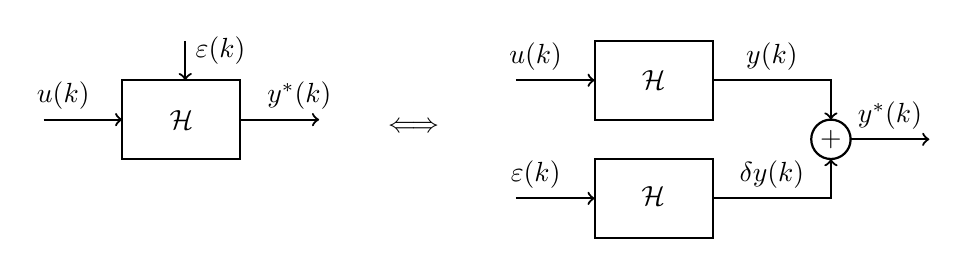
\begin{tikzpicture}[x=1cm,y=1cm]
				\draw (-9, 0.5) -- (-8,0.5) [->, thick] node[above,near start]{$\boldsymbol{u}(k)$};
				\draw (-7.2, 1.5) -- (-7.2,1.0) [->, thick] node[right,near start]{$\boldsymbol{\varepsilon}(k)$};
				\draw (-6.5, 0.5) -- (-5.5,0.5) [->, thick] node[above,near end]{$\boldsymbol{y}^*(k)$};
				\draw (-8,0.0) rectangle ++(1.5,1)[thick] node [midway]{$\mathcal{H}$}; 
				\draw (-2,0.5) rectangle ++(1.5,1)[thick] node [midway]{$\mathcal{H}$}; 
				\draw (-3, 1) -- (-2,1) [->, thick] node [above,near start]{$\boldsymbol{u}(k)$}; 
				\draw (-0.5, 1)  -- (1,1) -- (1,0.5) [->, thick] node[xshift=-0.75cm,yshift=0.8cm]{$\boldsymbol{y}(k)$}; 

				\draw (-2,-1) rectangle ++(1.5,1)[thick] node [midway]{$\mathcal{H}_{\abserr}$}; 
				\draw (-3, -0.5) -- (-2,-0.5) [->, thick] node[above,near start]{$\boldsymbol{\varepsilon}(k)$};
				\draw (-0.5, -0.5) -- (1,-0.5) -- (1,0) [->, thick] node [xshift=-0.75cm,yshift=-0.2cm]{$\boldsymbol{\delta y}(k)$}; 

				\draw (1,0.25) circle (0.25) [thick] node {$+$}; 
				\draw (1.25,0.25) -- (2.25,0.25)[->, thick] node [above,midway] {$\boldsymbol{y}^*(k)$};

				\node (arrow) at (-4.3,0.4) {$\iff$};
			  \end{tikzpicture}

			\caption{A signal view of the error propagation with respect to the ideal filter \label{fig:ltierror}}
			\end{figure}


		According to \ref{zmatrix}, we have:

		\begin{equation} \label{zepsmatrix}
		\boldsymbol{Z_\varepsilon}=
					\begin{pmatrix}
						\boldsymbol{-J} & \boldsymbol{M} & \boldsymbol{M}_t \\
						\boldsymbol{K} & \boldsymbol{P} & \boldsymbol{M}_x \\
						\boldsymbol{L} & \boldsymbol{R} & \boldsymbol{M}_y 
					\end{pmatrix}
		\end{equation}

		with:
		\begin{eqnarray} \label{deltaerr}
			\boldsymbol{M}_t=(\boldsymbol{I}_{n_t} \boldsymbol{0}_{n_t \times n_x} \boldsymbol{0}_{n_t \times n_y}), \\
			\boldsymbol{M}_x=(\boldsymbol{0}_{n_x \times n_x} \boldsymbol{I}_{n_x} \boldsymbol{0}_{n_x \times n_y}), \\
			\boldsymbol{M}_y=(\boldsymbol{0}_{n_y \times n_t} \boldsymbol{0}_{n_y \times n_x} \boldsymbol{I}_{n_y}),
		\end{eqnarray}

		$\mathcal{H}_{\boldsymbol{\varepsilon}}$ is a filter with ($n_t+n_x+n_u$) inputs and $n_y$ outputs.
		\begin{proposition}
			The transfert function of filter $\mathcal{H_{\boldsymbol{\varepsilon}}}$, denoted $\boldsymbol{H}_\varepsilon$, is defined as follows:
			\begin{equation}
				\boldsymbol{H}_{\varepsilon}: \rightarrow \boldsymbol{C_Z}(z\boldsymbol{I}_n-\boldsymbol{A_Z})^{-1}\boldsymbol{M}_1 +\boldsymbol{M}_2 \hspace{5pt} \forall z \in \mathbb{C}
			\end{equation}
			with $\boldsymbol{A_Z}$ and $\boldsymbol{C_Z}$ the matrices defined by \ref{abcdtranspose} and
			\begin{equation}
				\boldsymbol{M_1}=(\boldsymbol{KJ}^{-1}   \hspace{10pt}\boldsymbol{I}_{n_x} \hspace{10pt} \boldsymbol{0}), 
				\boldsymbol{M_2}=(\boldsymbol{LJ}^{-1}  \hspace{10pt}\boldsymbol{0} \hspace{10pt}\boldsymbol{I}_{n_y}), 
			\end{equation}
		\end{proposition}
		The demonstration is well detailed in Lopez' phd.

		\begin{corollary} \label{corimp}
			Considering a filter $\mathcal{H}$, $\boldsymbol{\varepsilon}(k)$ the vector of computation errors at time k in the finite precision of $\mathbb{H}$,
			and $\mathcal{H}\boldsymbol{\varepsilon}$ the error filter associated to $\mathcal{H}$.
			The behaviour of error can be described from $\boldsymbol{\varepsilon}(k)$ and $\mathcal{H}\boldsymbol{\varepsilon}$.
			Considering the error as an interval vector, denoted $\langle \boldsymbol{\varepsilon}_m, \boldsymbol{\varepsilon}_r \rangle$,
			the interval vector of global error $\boldsymbol{\delta y}$, denoted $\langle \boldsymbol{\delta y}_m, \boldsymbol{\delta y}_r \rangle$, is given by:
		\end{corollary}

		\begin{eqnarray} \label{eqprec}
			\boldsymbol{\delta y}_m = \langle\langle \mathcal{H}_{\boldsymbol{\varepsilon}} \rangle\rangle_{DC} \cdot \boldsymbol{\varepsilon}_m \\
			\boldsymbol{\delta y}_r = \langle\langle \mathcal{H}_{\boldsymbol{\varepsilon}} \rangle\rangle_{wcpg} \cdot \boldsymbol{\varepsilon}_r
		\end{eqnarray}

		In practise, the interval arithmetic comes from the command community.
		In signal community, and moreover in computer arithmetics, we are used to compute on intervals centered around zero.
		Then, we can reasonably deduce that DC-gains are null, so the previous solution gives:

		\begin{eqnarray} \label{eqprec}
			\boldsymbol{\delta y}_m = 0 \\
			\boldsymbol{\delta y}_r = \langle\langle \mathcal{H}_{\boldsymbol{\varepsilon}} \rangle\rangle_{wcpg} \cdot \boldsymbol{\varepsilon}_r
		\end{eqnarray}

		For the same reason (centered around zero), the interval becomes:
		\begin{eqnarray} \label{eqprec}
			\boldsymbol{\delta y}_m = -\langle\langle \mathcal{H}_{\boldsymbol{\varepsilon}} \rangle\rangle_{wcpg} \cdot \boldsymbol{\varepsilon}_r \\
			\boldsymbol{\delta y}_r = \langle\langle \mathcal{H}_{\boldsymbol{\varepsilon}} \rangle\rangle_{wcpg} \cdot \boldsymbol{\varepsilon}_r
		\end{eqnarray}

		Then, following Lopez's computations, we can derivate precisions for every intermediate step:
		
		\begin{equation}
			|\boldsymbol{\delta y}_i| \leq \sum_{j=1}^{n'} | \langle\langle \mathcal{H}_{\boldsymbol{\varepsilon}} \rangle\rangle_{i,j}| \cdot \boldsymbol{2^{l_{v'_j}}}
		\end{equation}

		To formalize with a matricial formulation, we get:
		\begin{equation}
			|\boldsymbol{\delta y}| \leq | \langle\langle \mathcal{H}_{\boldsymbol{\varepsilon}} \rangle\rangle| \cdot \boldsymbol{2^{l_{v'}}}
		\end{equation}

		\TODO: define or replace v









	\subsection{Adjustments in arbitrary precision}

	





%		
%	\subsection{Canonical specification}
%		
%		The intuitive and first way to describe an LTI filter is to specify the output as a function of the inputs:
%		$$y(k)=\sum_{i=0}^n b_i u(k-i)-\sum_{i=1}^n a_i y(k-i)$$
%
%	\subsection{Z transform}
%	$$X(z)=\mathcal{Z}\{x\}=\sum_{k=0}^{+\infty} x(k) z^{-k}$$
%	
%	\subsection{Transfert Function}
%	A filter is usually described by it's transfert function, defined as:
%
%	$$H(z)=\frac{Y(z)}{U(z)}=\frac{\sum_{i=0}^n b_i z^{-i}}{ 1 + \sum_{i=1}^n a_i z^{-i}}, \;\;\;\; \forall z \in \mathbb{C}$$ 
%	\subsection{Impulse response}
%	$\delta$
%	\subsection{Worst case peak gain (WCPG)}
%	$$\| \mathcal{H} \|_{WCPG}=\sup_{i\neq 0} \frac{\|h*u\|_{l^\infty}}{\|u\|_{l^\infty}} $$
%
%	$$\| \mathcal{H} \|_{WCPG}= \sum_{k \geq 0} |h(k)| $$
%	\subsection{Realisations}



	



